\documentclass{eecslides}
\usepackage{amsmath}
\usepackage{color}
\usepackage{listings}
\usepackage{url}
\definecolor{lgray}{gray}{0.9}
\lstset{ %
language=R,                		% choose the language of the code
basicstyle=\tiny,       % the size of the fonts that are used for the code
numbers=left,                  	% where to put the line-numbers
numberstyle=\footnotesize,   % the size of the fonts that are used for the line-numbers
stepnumber=1,                   	% the step between two line-numbers. If it is 1 each line will be numbered
numbersep=5pt,                  	% how far the line-numbers are from the code
backgroundcolor=\color{lgray},  % choose the background color. You must add \usepackage{color}
showspaces=false,              	% show spaces adding particular underscores
showstringspaces=false,         % underline spaces within strings
showtabs=false,                 	% show tabs within strings adding particular underscores
frame=single,           		% adds a frame around the code
tabsize=2,          			% sets default tabsize to 2 spaces
captionpos=b,           		% sets the caption-position to bottom
breaklines=true,        		% sets automatic line breaking
breakatwhitespace=false,    	% sets if automatic breaks should only happen at whitespace
escapeinside={\%*}{*)}          	% if you want to add a comment within your code
}
\setbeamertemplate{enumerate items}[default]
%------------------------------

\title[Stochasticity]{Stochastic models in ecology}
\subtitle{Analytical and numerical methods}
\author[D. Gravel]{Dominique Gravel}
\institute[Chaire de recherche EEC]{UQAR -- Chaire de Recherche EEC}
\website{http://www.chaire-eec.uqar.ca/}
\date{\today}

\begin{document}

	\begin{frame}[plain]
		\titlepage
	\end{frame}

	\begin{frame}[plain]{Outline}
		\tableofcontents
	\end{frame}

%------------------------------
%------------------------------

	\section{Introduction}

	\begin{frame}{Stochasticity in natural systems}

	Most biological processes are inherently stochastic, yet much theoretical analysis involves deterministic models. Why?\\
	\vskip 1em 

	\begin{itemize}
		\item Pragmatic reason: deterministic models are relatively easier to solve
		\item Biological systems typically consist of a large collection of individuals experiencing the same ecological interactions (assumes that the dynamics of the average is a sufficient description of the system)
	\end{itemize}
	\vskip 1em

	The question then is \emph{when does stochasticity matters and why?} 
	\end{frame}

%------------------------------

	\begin{frame}{Is the average enough?}

	Consider populations A and B with the same initial density (100 individuals in each one). If the growth rate of population A at year 1 is $\lambda_A (1) = 1$ and at year 2 is  $\lambda_A (2) = 2$, what is the population size after year 2? If the growth rate for population B is $\lambda_B(1) = 1.5$ and $\lambda_B(2) = 1.5$? Why is there a difference?

	\end{frame}
%------------------------------

	\begin{frame}{Is the average enough?}

	Program a stochastic version of the geometric growth model (discrete time) where $\lambda (t) = \mu + \epsilon (t)$, where $\epsilon (t)$ is a normal random deviate of mean 0 and variance $sigma^2$. \\
	\vskip 1em
	Start with $N_0 = 10$ and consider $\overline{\lambda} = 1.05$. Increases the variance of $\epsilon (t)$ by steps of 0.01 and for each level run 100 replicated simulations over 100 time steps. Plot the average population size and the number of extinctions as a function of the variance. 

	\end{frame}

%------------------------------

	\section{Objectives}

	\begin{frame}{Conceptual objectives}

	\begin{enumerate}
		\item Demographic stochasticity
		\item Environmental stochasticity
		\item Jansen's inequality
		\item Storage effect
	\end{enumerate}

	\end{frame}

%------------------------------

	\begin{frame}{Technical objectives}

	\begin{enumerate}
		\item Playing with random numbers
		\item Introduction to common algorithms
		\item Adding stochasticity to discrete time models
		\item Stochastic models
		\item Common probability distribution 
	\end{enumerate}

	\end{frame}

%------------------------------
	\begin{frame}[fragile]{Before the theory}{Essential programming tips}

		\begin{lstlisting}
		# Draw a random number between 0 and 1
		rand = runif(n = 1, min = 0, max = 1)

		# Set the seed of the random number generator
		set.seed(1)
		runif(n = 1, min = 0, max = 1)
		runif(n = 1, min = 0, max = 1)

		set.seed(1)
		runif(n = 1, min = 0, max = 1)
		runif(n = 1, min = 0, max = 1)

		# Draw a random event A with probability p 
		test = 0
		test[runif(n = 1, min = 0, max = 1) < p] = 1 
		
		# or alternatively
		if(runif(1,0,1) < p) test = 1 
		else test = 0

		\end{lstlisting}

	\end{frame}
%------------------------------
%------------------------------

	\section{Theory}

	\begin{frame}{Jensen's inequality}

		\begin{columns}
			\begin{column}{0.5\textwidth}		

			The principle: \\
			$f(\overline{x}) \neq \overline{f(x)}$
			\vskip 1em

			Consequences:\\
			\begin{itemize}
				\item $\overline{f(x)}>f(\overline{x})$ if the function is concave;
				\item $\overline{f(x)}<f(\overline{x})$ if the function is convex;
				\item $\overline{f(x)} = f(\overline{x})$ if the function linear;	
			\end{itemize}

			\end{column}
%----
			\begin{column}{0.5\textwidth}
				\begin{center}
					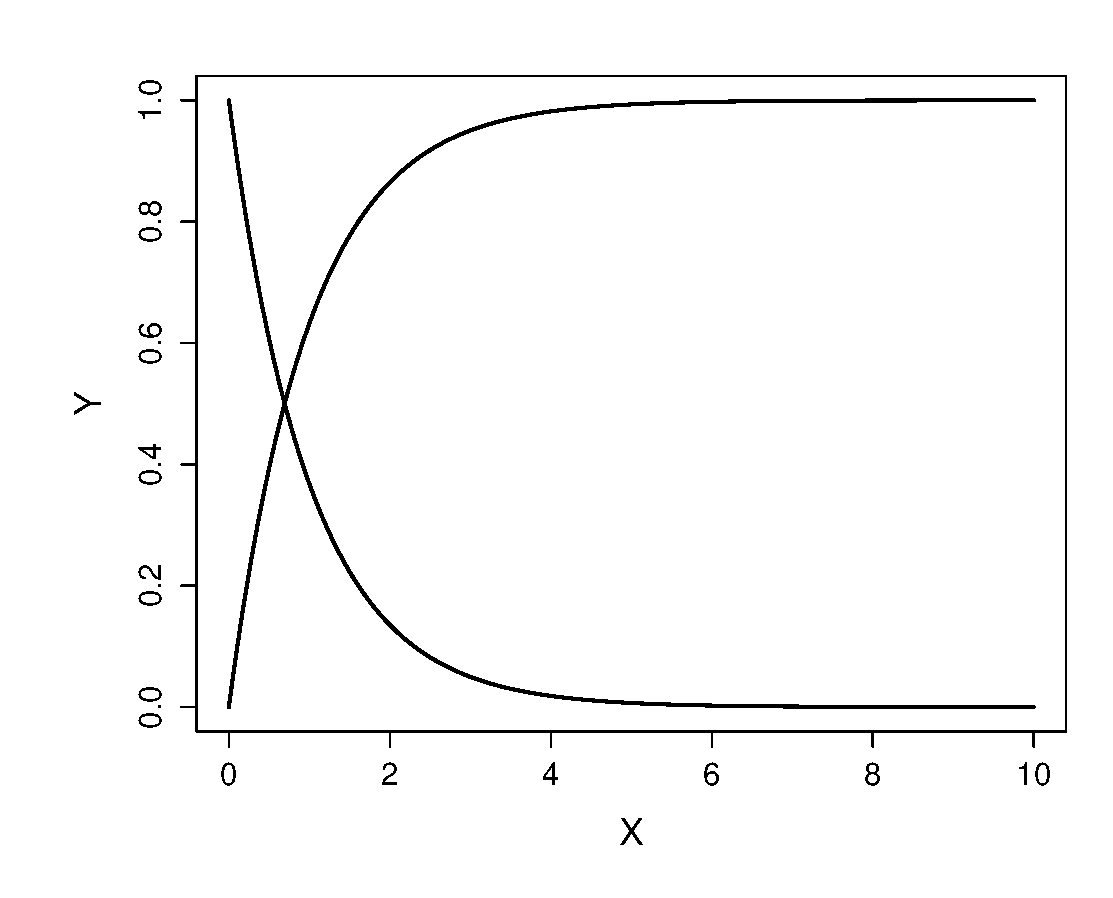
\includegraphics[height=0.5\textheight]{nonlinear.eps}
				\end{center}
			\end{column}
		\end{columns}	 

	\end{frame}

%------------------------------

	\begin{frame}{Jensen's inequality}{Examples}

		\begin{center}
			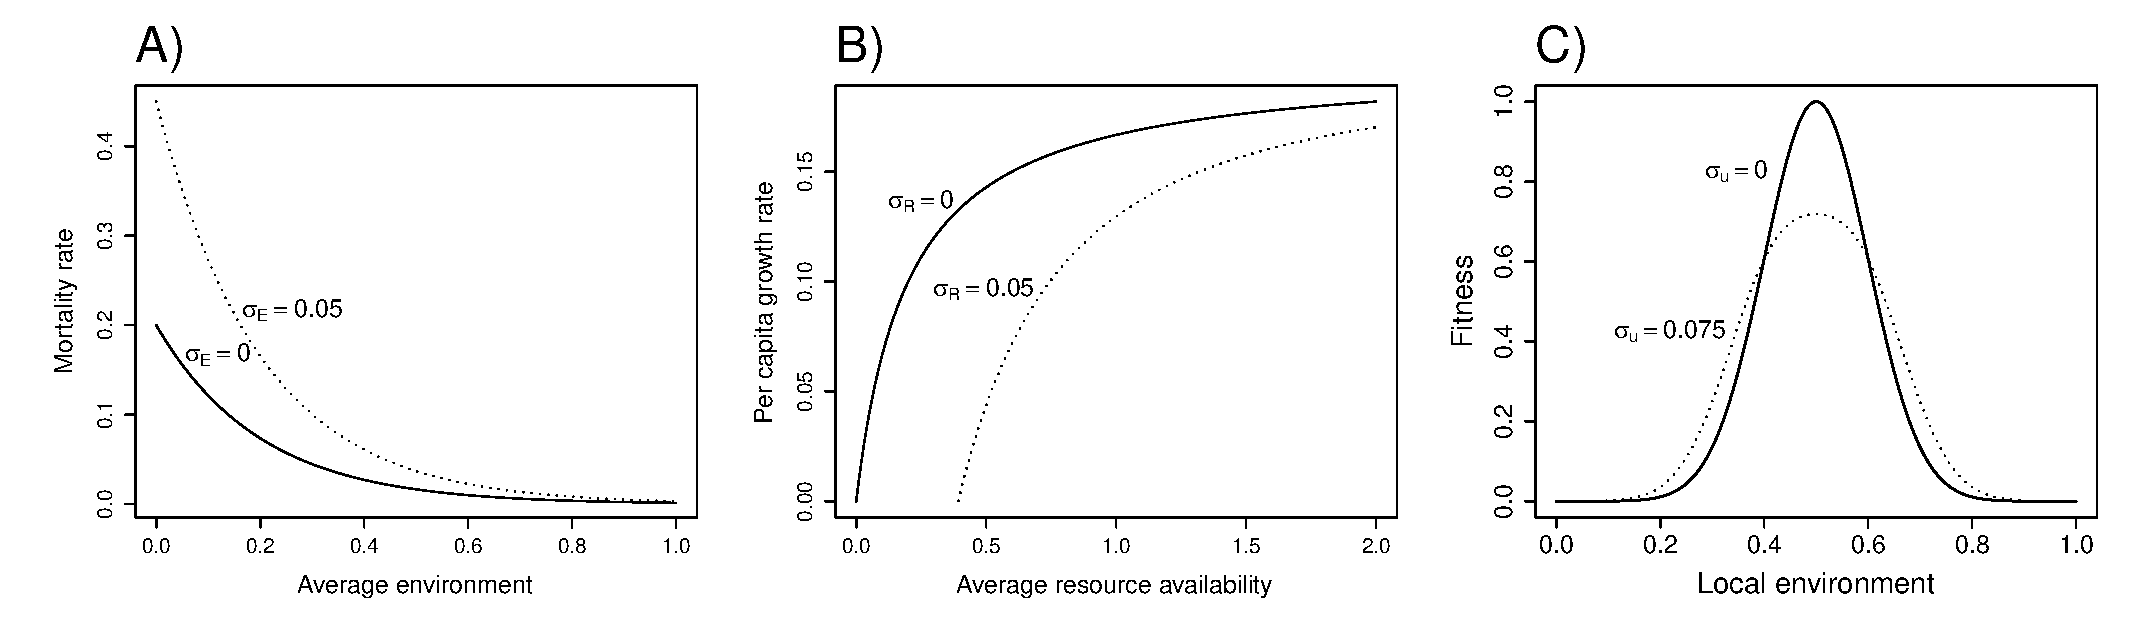
\includegraphics[height=0.35\textheight]{example_nonlinear.eps}
		\end{center}

	\end{frame}
%------------------------------

	\begin{frame}{Jensen's inequality}

		\begin{columns}
			\begin{column}{0.5\textwidth}		

			Computing the average of a non-linear function with the Taylor expansion:\\
			$ f(x+\epsilon) \approxeq f(x) + \frac{f'(x)(x-\epsilon)}{1!} + \frac{f''(x)(x-\epsilon)^2}{2!}+....$
			\vskip 1em

			Computing it over several measurements:\\
			$ \overline{f(x)} \approxeq f(\overline{x}) + \frac{f''(\overline{x})\sigma^2}{2}$

			\end{column}
%----
			\begin{column}{0.5\textwidth}
				\begin{center}
					\includegraphics[height=0.5\textheight]{taylor_approx.png}
				\end{center}
			\end{column}
		\end{columns}	 

	\end{frame}

%------------------------------

	\begin{frame}{Environmental stochasticity}{Expected long term average}

		Solution to the geometric growth model\\
		$N_{t+n} = N_0\lambda^n$\\
		$log(N_{t+n}) = log(N_0)+nlog(\lambda)$
		\vskip 1em

		Estimating the average population size:\\
		$\overline{log(N_{t+n})}=log(N_0)+nlog(\overline{\lambda})-\frac{n\sigma_{\lambda}^2}{2\lambda^2}$
		\vskip 1em

		\textbf{Exercise:} Calculate the maximal variance that a population of 100 individuals can stand if it has a groth rate of 1.025

	\end{frame}

%------------------------------

	\begin{frame}{Solution}

		\begin{columns}
			\begin{column}{0.45\textwidth}		

				Long-term average trajectory:\\
				$\overline{log(N_{t+n}}=log(N_0)+nlog(\overline{\lambda})-\frac{n\sigma_{\lambda}^2}{2\lambda^2}$
				\vskip 1em
	
				To solve the problem, we consider there is no change on average in population size, and therefore:\\
				$nlog(\overline{\lambda})=\frac{n\sigma_{\lambda}^2}{2\lambda^2}$
				\vskip 1em

				Isolating the variance term:\\
				$\sigma_{\lambda}^2=2\overline{\lambda}^2log(\overline{\lambda})$
				$\sigma_{\lambda}^2=0.0519$

			\end{column}
%----
			\begin{column}{0.55\textwidth}
				\begin{center}
					\includegraphics[height=0.5\textheight]{series_geometric.png}
				\end{center}
			\end{column}
		\end{columns}	 

	\end{frame}

%------------------------------

	\begin{frame}{Application of Jensen's intequality}{Relative non-linearity}

		Consider the problem of coexistence underlined by Armstrong and McGehee (1980). The community is made of two consumers (predators, $P_1$ and $P_2$) competing for a single resource (the prey, $N$). The dynamics are given by the following system of equations:\\

	$\frac{dN}{dt} = N(1-N)- \frac{a_1P_1N}{1+b_1N}- \frac{a_2P_2N}{1+b_2N}$\\
	$\frac{dP_1}{dt} = \frac{a_1P_1N}{1+b_1N} - m_1P_1$\\
	$\frac{dP_2}{dt} = \frac{a_2P_2N}{1+b_2N} - m_2P_2$\\
	\vskip 1em

		\begin{itemize} 
			\item What is the equilibrium N in presence of only one predator?
			\item If we consider $a_1 = 1$, $a_2 = 1$, $b_1 = 10$, $b_2 = 0$, $m_1 = 0.05$ and $m_2 = 0.2$, which species should win competition?
			\item Now run simulations of the model. Which species wins competition? Why?
		\end{itemize}

	\end{frame}

%------------------------------

	\begin{frame}{Intrinsic variability}{Relative non-linearity}

	Now we have an explanation for the coexistence observed in the Vandermeer (2006) paper. The mechanism is the \emph{relative non-linearity}.\\
		\begin{center}
			\includegraphics[height=0.5\textheight]{chesson_relnonlinear.png}
		\end{center}
		
		\begin{center}
			\centering \large{$\overline{r_i}\approxeq b_i(k_i-k_s)-b_i(\tau_i-\tau_s)V(F^{-i})$}
		\end{center}
	\end{frame}

%------------------------------

	\begin{frame}{Logistic growth}{Equilibrium population size}

		Consider a simple discrete time birth-death model:\\
		$N_{t+\Delta t} = N_t + [B(N) - D(N)]\Delta t + \Delta Z$\\
		\vskip 1em

		Because additive terms are satistically independent, the ensemble average yields:\\
		$\langle N_{t+\Delta t}\rangle  = \langle N_t\rangle  + [\langle B(N)\rangle  - \langle D(N)\rangle ]\Delta t + \langle \Delta Z\rangle $\\
		\vskip 1em

		Because we are interested by the equilibrium and on average $\langle \Delta Z\rangle = 0$, \\
		$\langle N_{t+\Delta t}\rangle = \langle N_t\rangle$
		\vskip 1em

		And therefore we are left with:\\
		$\langle B(N)\rangle  = \langle D(N)\rangle $
		
	\end{frame}

%------------------------------

	\begin{frame}{Logistic growth}{Equilibrium population size}
	
		So if we are now more specific about B and D, using the logistic growth model, we have:\\
		$\langle(a_1N-b_1N^2)\rangle = \langle(a_2N-b_2N^2)\rangle$\\
		$a_1\langle N \rangle - b_1 \langle N^2 \rangle = a_2\langle N \rangle - b_2 \langle N^2 \rangle$
		\vskip 1em

		Collecting terms:\\
		$(a_1-a_2)\langle N \rangle = (b_1 + b_2) \langle N^2 \rangle$
		\vskip 1em

		If we now define the mean, $m = \langle N \rangle$, and variance, $V(N) = \langle N^2 \rangle - m^2$, we have:\\
		$(a_1-a_2)m = (b_1+b_2)(V(N)+m^2)$\\
		$m = \frac{a_1-a_2}{b_1+b_2}-\frac{V(N)}{m}$\\
		$m \approxeq \frac{r}{s} - \frac{s}{r}V(N)$\\
		\vskip 1em

		where $r = a_1-a_2$ and $s = b_1+b_2$. The approximation assumes a small variance-to-mean ratio. The stochastic mean collapses to the deterministic expectation as $V(N)$ tends to 0. 

	\end{frame}
%------------------------------

	\begin{frame}{Demographic stochasticity}

		Birth and death are discrete events inherently variable, independently of environmental stochasticity. If we consider the population growth rate $\lambda$ as an average of individual probabilities of birth and death, $\omega$, we have: \\
		$\lambda = \overline{\omega}$\\
		$\lambda = \frac{1}{N}\sum \omega_i = \mu_\omega + \frac{1}{N} \sum \delta_i$
		\vskip 1em

		where $\mu$ is the population average and $\delta_i$ are individual differences to this average. \\
		\vskip 1em

		Now taking the variance of the population growth rate we obtain:\\
		$\sigma_{\lambda}^2 = Var[\mu_\omega]+ \frac{1}{N^2} \sum Var[\delta_i]$\\
		$\sigma_{\lambda}^2 = \sigma_e^2 + \frac{\sigma_d^2}{N}$\\
		\vskip 1em

		In ecological terms: the impact of demographic stocahsticity on the variability of the population growth rate shrinks asymptotically to 0 with large population size. 

	\end{frame}

%------------------------------

	\begin{frame}{Coexistence in a variable world}{Storage effect}

		The lottery model:\\
		$N_{1,t+1} = (1-d_1)N_{1,t}+(d_1N_{1,t}+d_2N_{2,t})\frac{f_1(t)N_{1,t}}{f_1(t)N_{1,t}+f_1(t)N_{1,t}}$
		\vskip 1em
		
		where $d_i$ is the probability of mortality (which we will assume equal for both species for simplicity) and $f_i(t)$ is the fecundity. The dependance of $t$ means that it could vary over time.\\
		\vskip 1em

		After some re-arrangement of this equation, we obtain the per capita growth rate of species 1 when an invader:\\
		$\frac{N_{1,t+1} }{N_{1,t}} =1+d[\frac{f_1(t)}{f_2(t)}-1]$
		\vskip 1em

		Reciprocal invasibility is impossible in absence of any variability (the per capita growth rate of the species with the smallest average $f$ will be lower than 1). 

	\end{frame}

%------------------------------

	\begin{frame}{Coexistence in a variable world}{Storage effect}

		Using the formula for long-term averaging we obtain:\\

		$\frac{\overline{N_{1,t+1}}}{\overline{N_{1,t}}} =1+d[\frac{\overline{f_1}}{\overline{f_2}}-1]+ d[\frac{\overline{f_1}}{\overline{f_2}^3}]\sigma_{f_2}^2$
		\vskip 1em

		The second derivative with respect to $f_2$ is positive, meanting that any variability in fecundity of species 2 will increase the growth rate of species 1 when at low abundance. \\
		\vskip 1em

		Ingredients for the storage effect:\\
		\begin{itemize}
			\item Differential response to the environment
			\item Covariance between environment and competition
			\item Buffered population growth
		\end{itemize}

	\end{frame}
%------------------------------

	\begin{frame}{Extinction probability}
		But the problem is that at low abundance, demographic stochasticity might play a role and kick-out the invader of the system, even it's long term average growth rate is positive.\\
		\vskip 1em

		With a fair amount of algebra, Cohen and Lewontin (1969) shown that the extinction risk for geometric growth is simply given by the integral of the normal distribution $G(\mu_x, \sigma_x^2/T)$ of the growth rate $x$ with mean $\mu_G$ and variance $\sigma_G^2/T$:\\
		$Pr(N_t<N_0) = \int G(x;\mu_G;\frac{\sigma_G}{\sqrt{T}})dx$
		\vskip 1em

		\textbf{Interpretation:} The probability of extinction\\

		\begin{itemize}
			\item Increases as the average per capita growth rate tends to zero
			\item Is a saturating positive function of the variance in the per capita growth rate
		\end{itemize}		
	
	\end{frame}

%------------------------------

	\begin{frame}{Coexistence in a variable world}{Drift versus storage effect}
		To understand the joint effects of stochasticity on coexistence, we now have to balance two potentially opposed forces:
		\begin{itemize}
			\item Stochasticity could promote the long term average population growth rate (- far from a rule though -)
			\item Stochasticity could increase the variance in population size, promote the drift and even random extinctions despite a positive growth rate.
		\end{itemize}	

	\end{frame}

%------------------------------

	\begin{frame}{Coexistence in a variable world}{Extinction versus storage effect}

		\begin{center}
			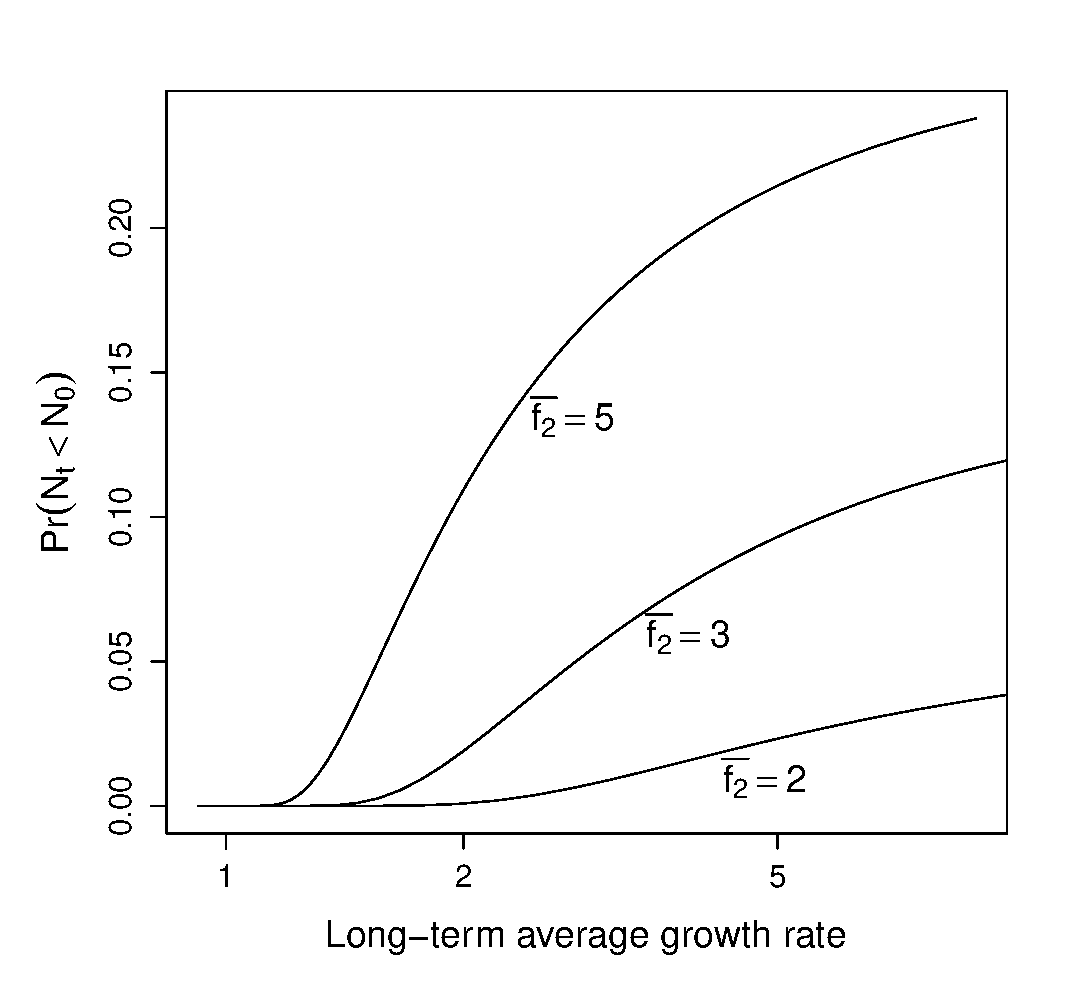
\includegraphics[height=0.7\textheight]{storage_extinction.eps}
		\end{center}

	\end{frame}

%------------------------------

	\begin{frame}{Coexistence in a variable world}{Drift versus stability}

		\begin{center}
			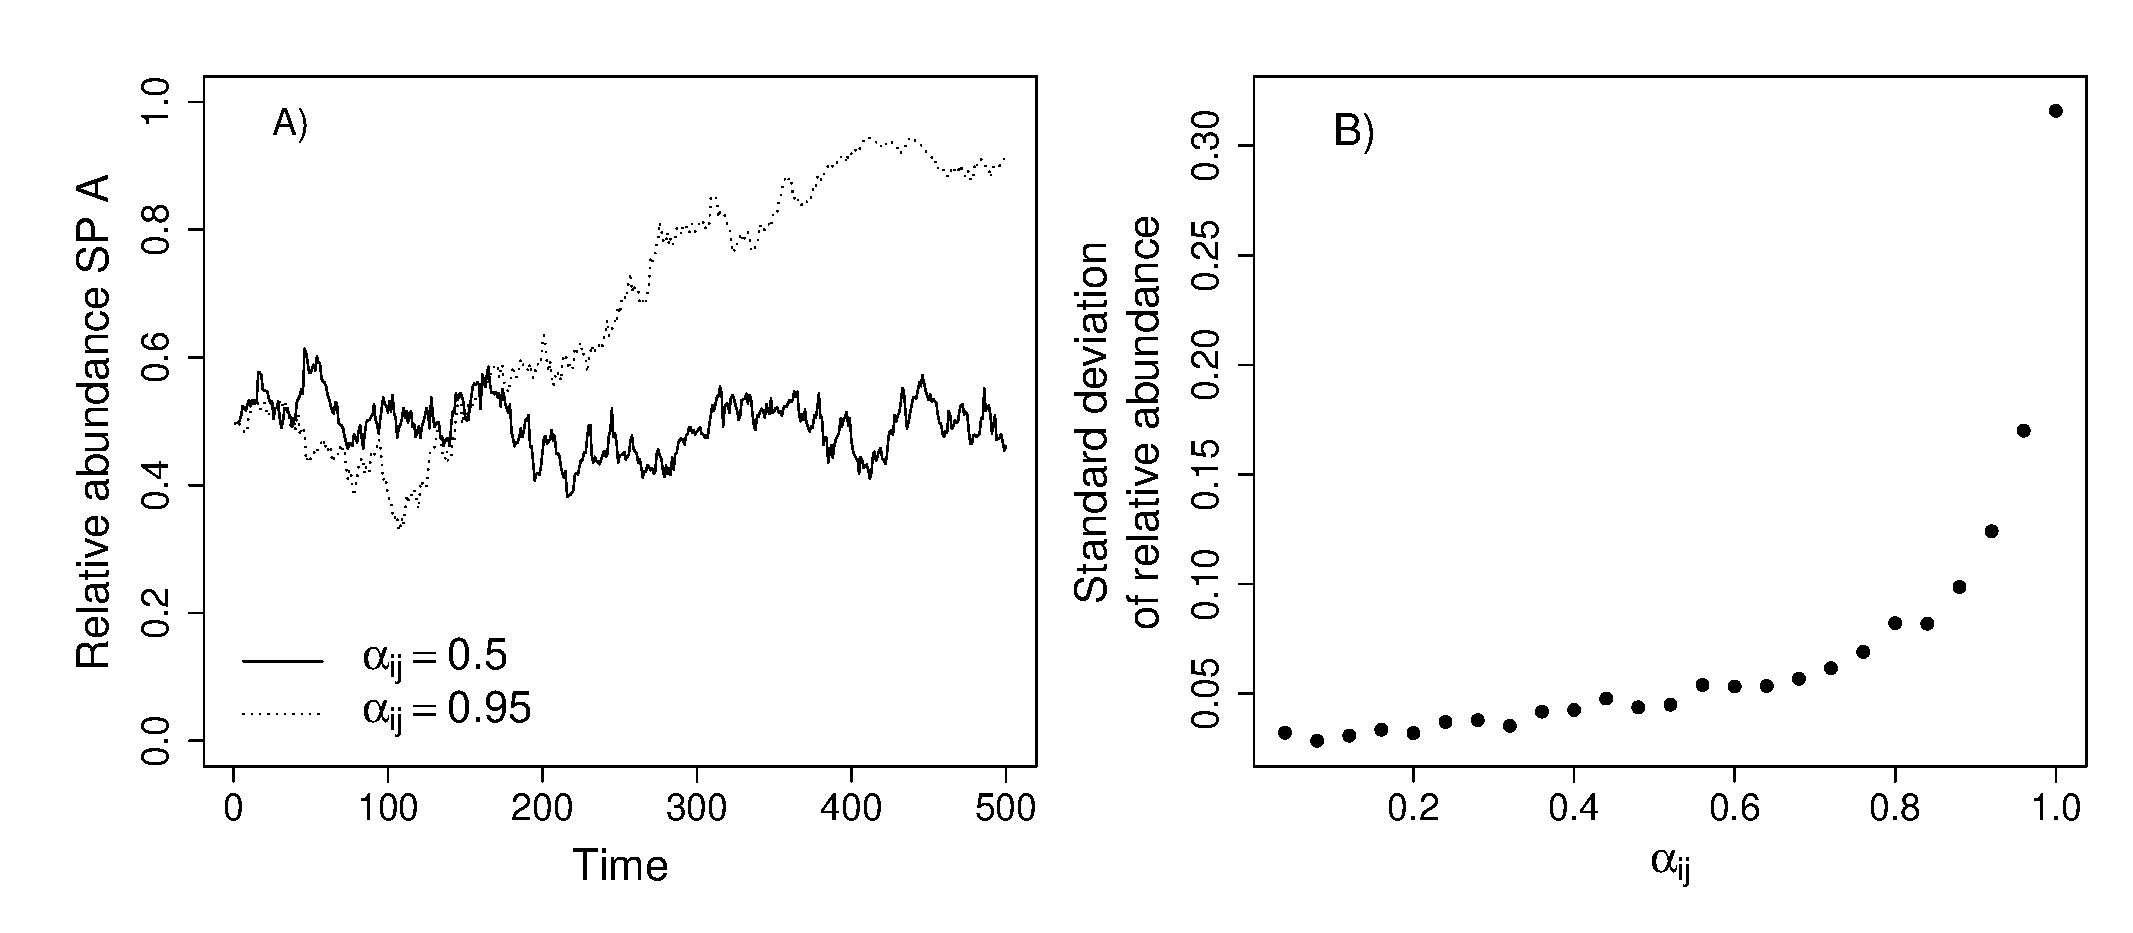
\includegraphics[height=0.5\textheight]{drift_stab.eps}
		\end{center}

	\end{frame}

%------------------------------

	\section{Stochastic models}

	\begin{frame}{Simulating stochastic models}{Project A: additive noise}

		\begin{center}
			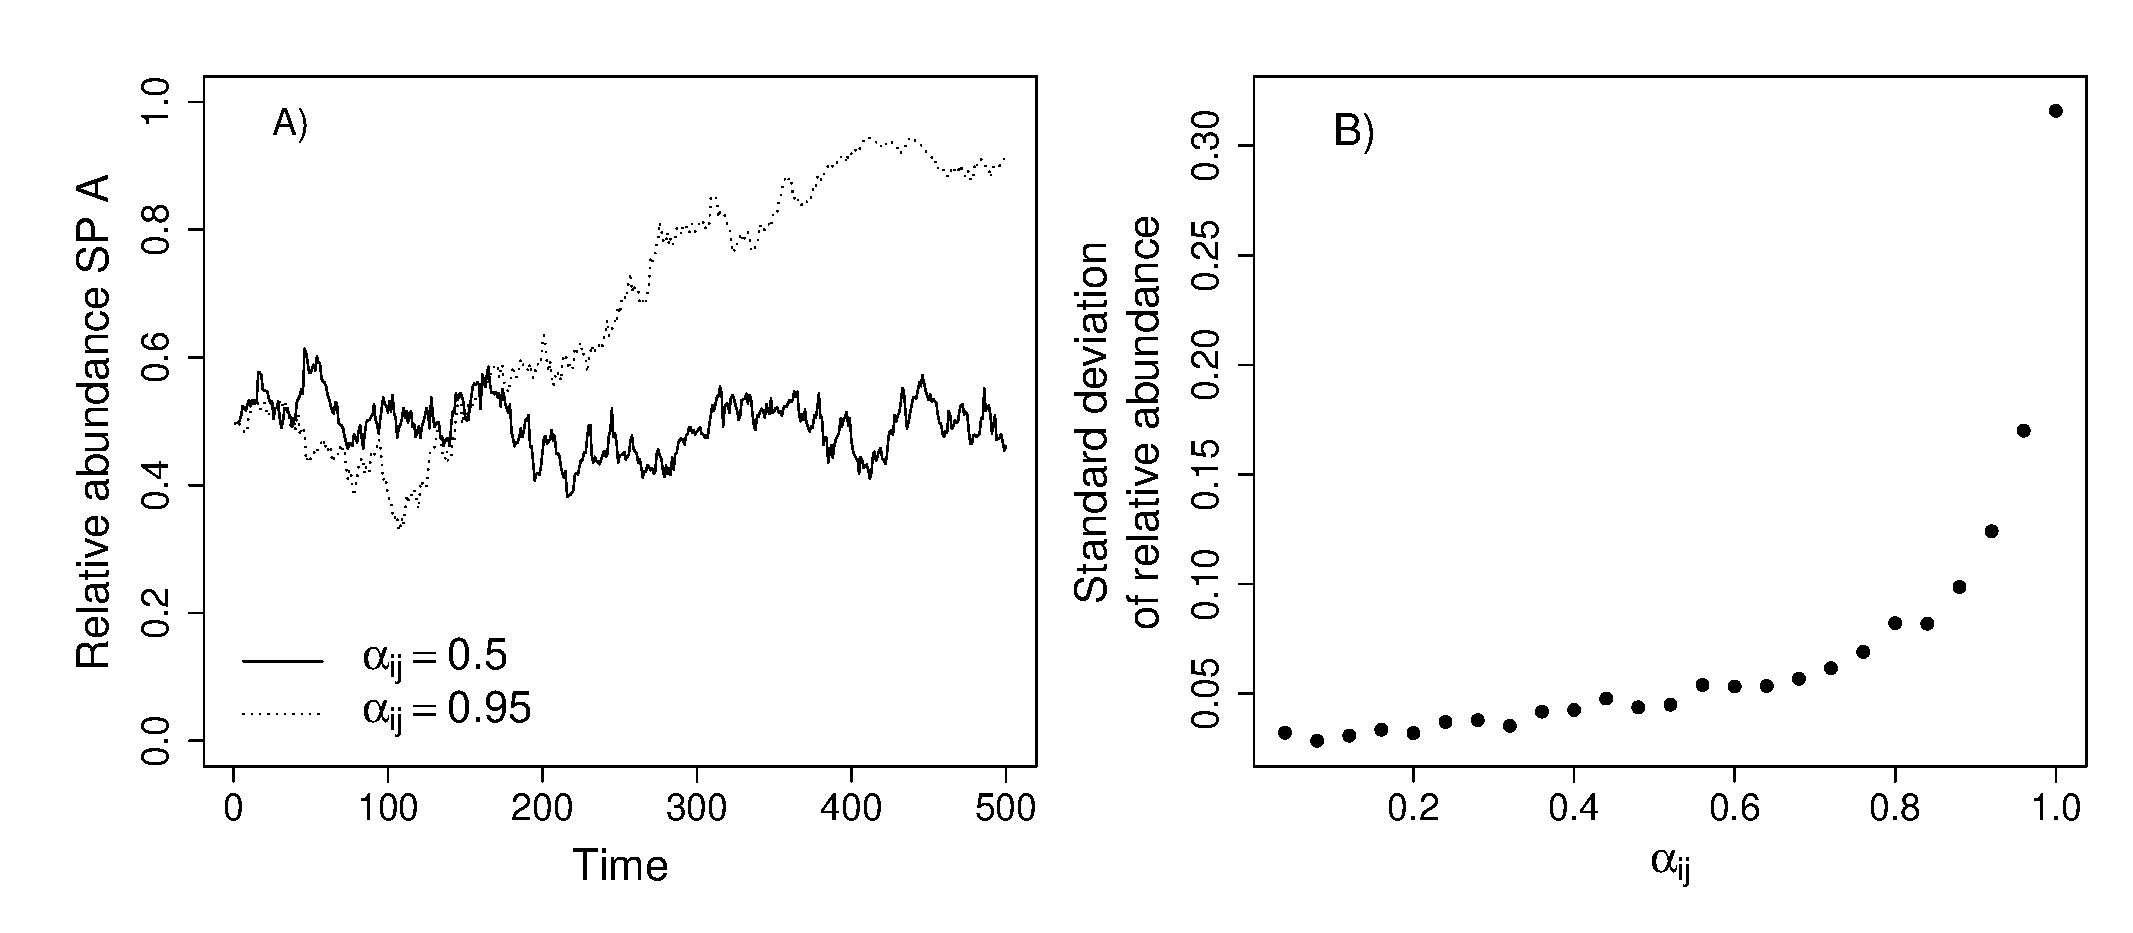
\includegraphics[height=0.4\textheight]{drift_stab.eps}
		\end{center}

\tiny{Ecological drift in a stable two species discrete version of the Lotka-Volterra model of competition. Environmental variability is introduced by independent normal random deviates to the carrying capacity of each species (mean of 0, standard deviation of 0.2). (a) Time series of species A relative abundance for weak ($a_ii = 1$ and $a_ij = 0.5$) and strong ($a_ii = 1$ and $a_ij = 0.95$) interactions. (b) Variability in species A relative abundance after 1000 time steps, based on 1000 replicated runs and as a funciton of the strenght of interspecific competition. Maximal variability occurs when there is systematix fixation (one species dominates and the other goes extinct). Parameters: $r_1 = r_2 = 1.24$, $K_1 = K_2 = 1$.}

	\end{frame}

%------------------------------

	\begin{frame}{Simulating stochastic models}{Project B: probabilistic models}

		Program an individual based lottery model. Consider a finite forest stand of 1 hectare, which holds approximately 250 adult trees. Recruitment follow a lottery: when an individual dies, with probability $d$, the identity of the recruited species is determined from a random draw among the seeds falling into the gap created by the death of the adult tree. Consider (fow now) global dispersal within this forest patch. Fecundity could vary among species and years. 

	\begin{itemize}
		\item Start with only 2 species and now environmental variation
		\item Add random variation in both species fecundity. 
		\item Vary the death probability instead of fecundity
		\item Now consider the possibility of 10 species. Plot the expected species richness as a function of the variance in fecundity.
	\end{itemize}

	\end{frame}

%------------------------------
%------------------------------

	\section{Useful algorithms}

%------------------------------

	\begin{frame}{Useful algorithms}{Exercise 1}

	Draw 10 random numbers from a uniform distribution. \\
	\begin{itemize}
		\item calculate the mean 
		\item calculate the variance
		\item find the largest and smallest values, without using min and max functions
		\item sort them
		\item find the median
		\item mix them again
		\item subsample 5 of them	
	\end{itemize}

	\end{frame}
%------------------------------

	\begin{frame}{Useful algorithms}{Exercise 1}
		
		\url{http://www.sorting-algorithms.com/}

	\end{frame}
%------------------------------

	\begin{frame}{Useful algorithms}{Exercise 2}

		The probabilities of observing events A, B and C are 0.2, 0.1 and 0.7, respectively. Program a function to draw one of these states randomly.

	\end{frame}

%------------------------------

	\begin{frame}{Useful algorithms}{Exercise 3}

	If probability of observing A is 0.3, observing B is 0.5 and the two are independent, what is the observing neither A nor B? observing 	both A and B?
	\vskip 1em

	Write a function drawing the event B if the probability of observing is 0.2 when A is observed and 0.8 when A is not observed. 
	\vskip 1em

	The probabilities of observing events A, B and C are 0.2, 0.1 and 0.7, respectively. Program a function to draw one of these states randomly.

	\end{frame}

%------------------------------

	\begin{frame}{Useful algorithms}{Exercise 4}

	Write a function to compute random numbers from a normal distribution based on a uniform random number generator
	\vskip 1em

	Idem but for an exponential random number generator

	\end{frame}

%------------------------------

\end{document}